\section{Introduction}

\subsection{Problem Definition}

\par Finding work in today’s economy can be a difficult process. There are so many services promising to help find a job but often times they just don’t pan out.  Building a professional LinkedIn profile, or typing up a resume and sending it out to employers could be motivating but if a person has lost their job or are simply in-between work, they might not have the time to wait. An online job portal system, also known as an online career board system, is a platform that helps job seekers find jobs and assists the employers in finding the best candidates. Online job portals offer a wide range of jobs in various numbers of fields. They are an important part of almost every hiring procedure, and using them efficiently will interpret into qualified candidates for moderately low costs. Even with the proliferation of digital recruiting tools, recruiting isn’t as easy as you’d expect it to be in the 21st century. If anything, finding qualified candidates is more challenging, complex and outright time-consuming. One of the biggest online recruiting challenges is an underwhelming number of applicants, which indicates a talent shortage and a consequence of the tight labor market, but it also signals that HR managers could benefit from expanding their recruiting tool sets. Lastly, without ample descriptions and carefully selected keywords, the right candidate will have a harder time finding the right position for them.

Many large organizations, government institutions, non-profit organizations, and private companies have their own job portals that job seekers directly access on their website, though it is quite common that most companies waste a lot of their resources, such as money and time to find the suitable candidates for their vacant positions. There are currently many job portal systems available but only a few of them interact with organizations and job seekers effectively. The ineffectiveness of most of the websites could present itself as being a hurdle for both parties’ recruitment process, such that organizations are spending a lot of time in finding the suitable candidate even after posting vacancy advert and employees should also wait a long time after applying for a job.

In the current market, the searches by candidates are not very elaborate and if the search does not return many results, then recall has to be high to keep the candidate engaged on the site. Thus, providing a personalized job search to candidates on the basis of their profiles and past search history makes sense for the candidates. On the recruiter side, the search provided over the candidate database is required to have a huge set of fields to search upon every data point that the candidate has entered. The recruiters are very selective when it comes to searching for candidates for specific jobs. Educational qualification, industry, function, key skills, designation, location, and experience are some of the fields provided to the recruiter during a search, which is why the precision should also be very high. 
\\
\par Having an effective recruitment process means starting with a clear understanding of what the business needs, then communicating that well to attract quality candidates, and carefully select the one who best meets those requirements. It’s more than just finding the most talented or qualified people. It’s about getting the right talent for the role and the company; people with the best possible skill-set and the right personality for the team and business. Every stage is important, from defining the job through to interviewing and reference-checking candidates, and the combined effectiveness determines whether the new employee will turn out to be an asset or a liability. High employee turnover can be a real problem for a company’s long-term prospects, but if the recruitment and selection processes are effective, the company will be far more likely to consistently pick people who perform well and remain loyal employees. An efficient, seamless recruitment experience increases the likelihood that new employees will be more engaged and motivated from the get-go, which improves their long-term chance of succeeding in the job and working to build the business. Quite apart from the effect of their own poor performance, hiring the wrong person can create stress and conflict in the team, and suck up management time that could be better spent on developing people and the business.

\subsection{Project Definition}

\par The project is designed to overcome some of the problems faced with the previous systems when it comes to job recruitment. The web application is proposed for both recruiter and candidate that enables them to navigate their needs in a focused and streamlined way. The service will be able to link up the person looking for a job to the right available position through search tags. The candidate uploads their CV to the platform in order for it to get parsed and tokenized. The recruiter will then be able to search their desired tags and find the right person for their company. Generally, the features are:

\begin{itemize}
    \item uploading a file and parsing it in order to tokenize it and create tags that describe specific attributes of the recruited
    \item target-searching an applicant through distinctive tags
    \item target-searching a company through distinctive tags
    \item communication between both parties through a private chat
\end{itemize}

The platform also provides an efficient way to pass the information between different users to cater their needs and enables corporate recruiters and job seekers to come under one roof. The website mainly aims on two kinds of users: \\

\textbf{A. Job Seekers} \\
Search jobs, post the CV which the system will parse and create a candidate profile, get matches based on the individual qualifications.

\textbf{B. Employers} \\
Post jobs, search resumes, screen candidates and streamline the entire hiring process, get matches based on the specified needs. \\

\textbf{Advantages:}

\begin{itemize}
    \item Faster and efficient system 
    \item Automatically creates a detailed and accurate profile
    \item Provides a facility for the Employer to search for required people very easily 
    \item Provides efficient search mechanisms
\end{itemize}

\subsection{Target Audience}

\par While the economy is recovering from the strong recession caused by the Covid-19 pandemic (GDP decline in 2020: -7\%, estimated growth in 2021: 4,5\%), the much-needed recovery of labour markets is lagging. According to ILO calculations, the country saw a decline in working hours of 8.7\% in 2020 (EU average 7.4\%) which is equivalent to 85,000 full time jobs. In 2021, the loss of working hours only slightly decreased and is still at 6.8\% (EU average 2.7\%), equivalent to the loss of 82,000 full-time jobs. 
\\
\par Thus, there is a national need for employment efficiency in the current market, which would mainly cater to the average worker. The proposed recruitment platform would cater to the typical unemployed person from Moldova, age 18 and above who are very passionate about their field of study and who are looking forward to share their knowledge with the world. Their main need would cover:

\begin{itemize}
    \item Wanting to find a fitting job for their expectations and their specific set of skills
    \item Wanting to use a website that scrapes jobs based on detailed skills
    \item Wanting to use a single website to look for a job
    \item Wanting a simple and intuitive way to look for a job
    \item Wanting to not waste a lot of time for the job searching process 
\end{itemize}

\par On the employer side, the platform will cater to locally based companies whose HR teams are looking for a digitized way to recruit qualified people for their open positions and who want to use a common platform that would scrape for their specific candidate needs.


\subsection{Comparison and SWOT Analysis}

\par In order to have a good understanding of what the market lacks, it is important to analyze what are the options presented when it comes to recruitment platforms. Thus, next up is the competitive analysis of the four most used web applications in Moldova for job seeking: 

\begin{enumerate}
    \item \textbf{Delucru.md} is an online platform where one can find thousands of jobs from all over the country. Every day employers publish dozens of job offers from different fields of activity on the website, such as: IT, medicine, finance and banking, sales, jobs for students, jobs abroad, jobs that don't require previous work experience etc. One can also choose the work schedule that suits you best - part time, full time or remote, create a CV right on the account or add it as a file.
    
    \textbf{Advantages:}
    \begin{itemize}
        \item Create a CV directly on the platform
        \item Intuitive UI design
        \item Has a separate blog about job trends
        \item Has the “Aplică rapid” option
        \item Can track the history of the applications
    \end{itemize}
    
    \textbf{Disadvantages:}
    \begin{itemize}
        \item Can’t create a custom user profile
    \end{itemize}
    
    
    \item \textbf{Rabota.md} is another website for job seeking and advertisement. According to the platform, registering and completing the CV takes about half an hour. Immediately after completing it, the user can send it to all potential employers whose vacancies published on the site interest them. The more applications – the more chances to find the desired job.
    
    \textbf{Advantages:}
    \begin{itemize}
        \item Has mobile app option
        \item Create CV directly on the platform
        \item Get notified on new positions
    \end{itemize}
    
    \textbf{Disadvantages:}
    \begin{itemize}
        \item Can’t create a custom user profile
        \item Can’t track your application status
    \end{itemize}
    
    
    \item \textbf{LinkedIn} is a social media website that many people use to find jobs, connect with colleagues and business partners, and stay up-to-date on industry news. Some of these key features include:
    
    \begin{itemize}
        \item A comprehensive profile system that allows users to list their skills, experience, education, and contact information
        \item The ability to search for other users based on specific criteria, such as job title, company size, or location
        \item A rich media platform that allows users to post articles, images, and videos
    \end{itemize}
    
    \textbf{Advantages:}
    \begin{itemize}
        \item Works as both a social and recruitment platform
        \item Create a comprehensive user profile
        \item Easy to search perspective companies 
        \item Great UI experience
        \item Get notifications about vacant jobs
    \end{itemize}
    
    \textbf{Disadvantages:}
    \begin{itemize}
        \item Not every company posts their free positions there
        \item Takes an extensive amount of time to create the user profile
        \item Can’t track the job application
    \end{itemize}
\end{enumerate}

\begin{longtable}[h!]
\centering
\label{table:swot}

\caption{SWOT Analysis.}
\endfirsthead

%\caption* {\textbf{Table \ref{table:swot} Continued:}}\\\toprule
%\endhead

%\endfoot
%\bottomrule
%\endlastfoot

    \begin{tabular}{|p{7.5cm}|p{7.5cm}|}
    \hline
    
    \textbf{Strengths:}
    
    \begin{itemize}
        \item Faster and efficient system 
        \item Automatically creates a detailed and accurate profile based on the uploaded CV
        \item Provides a facility for the Employer to search for required people very easily 
        \item Provides efficient search mechanisms
        \item Provides matches for the recruiter and applicant 
    \end{itemize}
    
    & \textbf{Weaknesses:}
    
    \begin{itemize}
        \item Does not have a separate blog about job trends
        \item Does not allow to create a CV on the website
    \end{itemize}
        
    \\ \hline
    \textbf{Opportunities:}
    
    \begin{itemize}
        \item Establish an effortless communication mean between the applicant and the recruiter 
    \end{itemize}
        
    & \textbf{Threats:} 
    
    \begin{itemize}
        \item Competitors with more resources for marketing
        \item Competitors with an established name on the market
        \item High costs for pushing the platform to the public
    \end{itemize}
         
    \\ \hline
    \end{tabular}
\end{longtable}

\clearpage

\section{Project Architecture}

\subsection{Architecture 4 + 1}

\par To describe current project, there was chosen "4+1" Architecture, which is a model consisted of 5 kinds of so-called views. The views are used to explain the system from the perspectives of various stakeholders, including project managers, end-users, developers, and system engineers. \\

\textbf{Process View}

\par In order to create simple for users platform, there was chosen path of adding basic or minimalist functionality, which will not disturb the user during app usage. The three most basic functionalities can be seen on the Activity Diagrams presented below: 

\graphicspath{img/}
\begin{center}
\label{diagram:activityEmployee}
	\begin{tabular}{ c }
		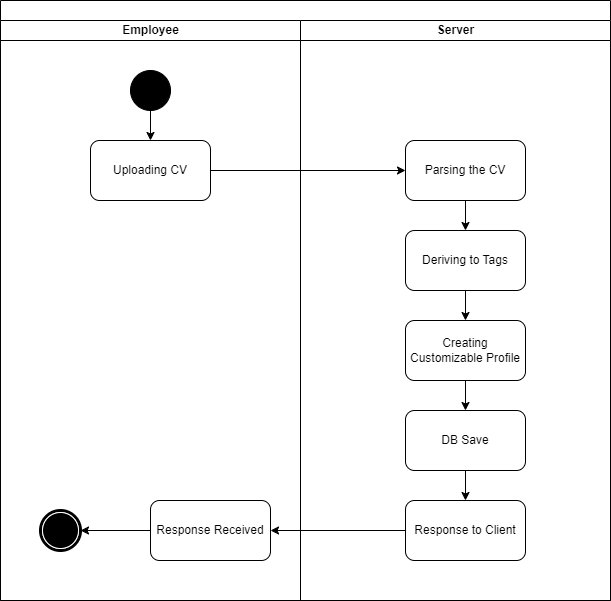
\includegraphics[scale = .75]{images/activityEmployee.png} \\
		Figure 2.1 - Activity UML Diagram from Employee Point of View
	\end{tabular}
\end{center}

\graphicspath{img/}
\begin{center}
\label{diagram:activityEmployer}
	\begin{tabular}{ c }
		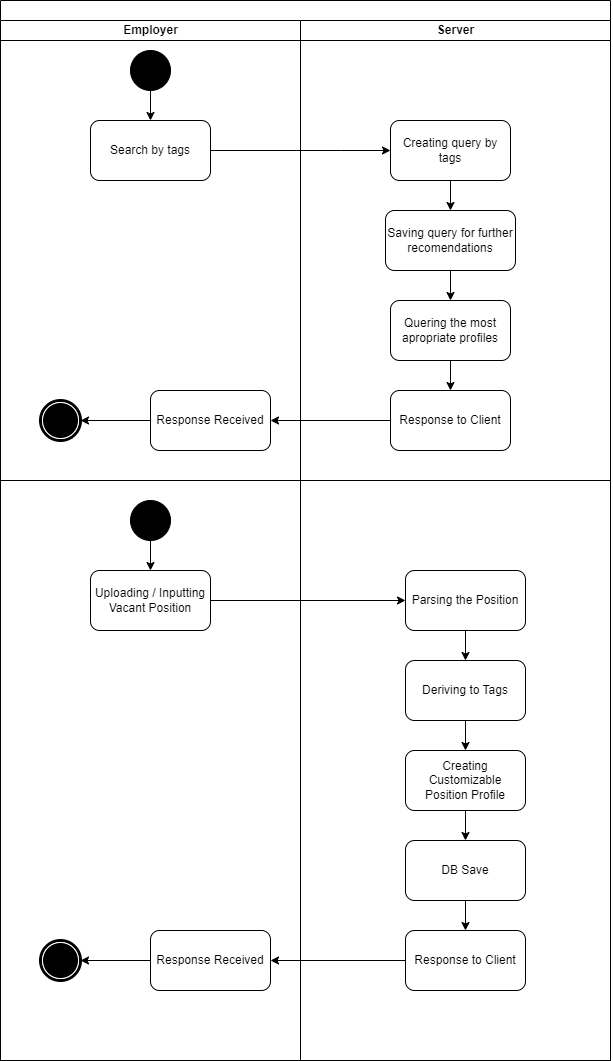
\includegraphics[scale = .65]{images/activityEmployer.png} \\
		Figure 2.2 - Activity UML Diagram from Employer Point of View
	\end{tabular}
\end{center}

\clearpage

\par Sequence diagrams shows how the system is responding to different type of requests. In our case, the most possible variant is to create asynchronous requests / response server to increase system responsiveness from the point of view of the users.

\graphicspath{img/}
\begin{center}
\label{diagram:sequenceEmployee}
	\begin{tabular}{ c }
		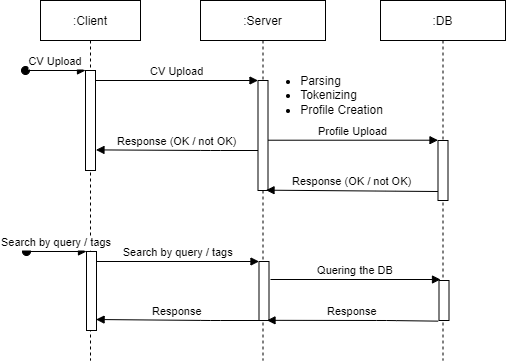
\includegraphics[scale = .8]{images/sequenceEmployee.png} \\
		Figure 2.3 - Sequence UML Diagram from Employee Point of View
	\end{tabular}
\end{center}

\graphicspath{img/}
\begin{center}
\label{diagram:sequenceEmployer}
	\begin{tabular}{ c }
		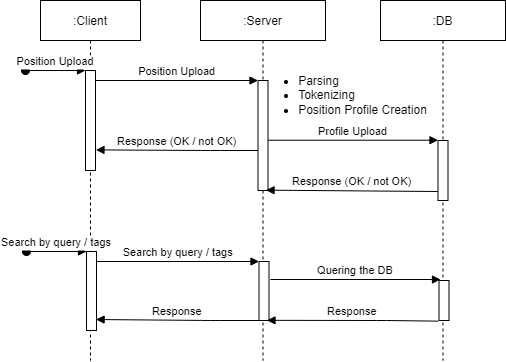
\includegraphics[scale = .8]{images/sequenceEmployer.png} \\
		Figure 2.4 - Sequence UML Diagram from Employer Point of View
	\end{tabular}
\end{center}

\clearpage

\textbf{Scenarios}

\par Of course, as it was mentioned before, the system should be minimalist, and the principal goal is to make it easy for the user. Below is presented Use Case Diagram for both types of Users: Employees and Employers:

\graphicspath{img/}
\begin{center}
\label{diagram:usecase}
	\begin{tabular}{ c }
		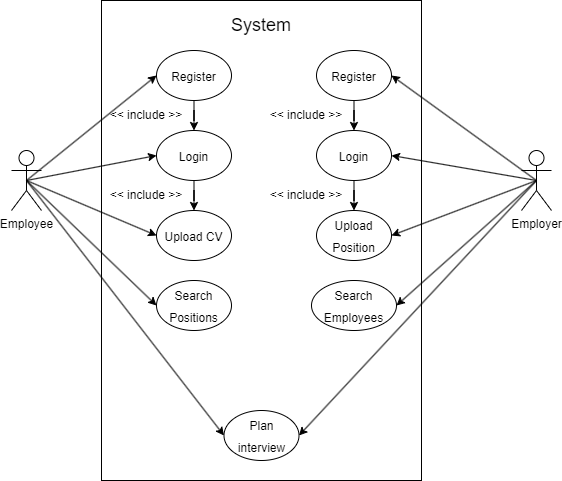
\includegraphics[scale = .8]{images/usecase.png} \\
		Figure 2.5 - Use Case Diagram of the whole System for current moment
	\end{tabular}
\end{center}